%29/01 - Fátima Sánchez Cabo
\chapter{Diseño experimental y principios estadísticos del análisis de datos ómicos}
El transcriptoma permite estudiar cómo se expresan los ARNs, incluyendo tanto ARNs codificantes (como los ARNm) como no codificantes (como microARNs, ARN de transferencia, etc.). El proteoma se centra en el estudio de las proteínas, que son los productos funcionales de muchos ARNm. Finalmente, el metaboloma estudia los metabolitos, que son los productos finales de las reacciones bioquímicas en las células.

\begin{figure}[h]
\centering
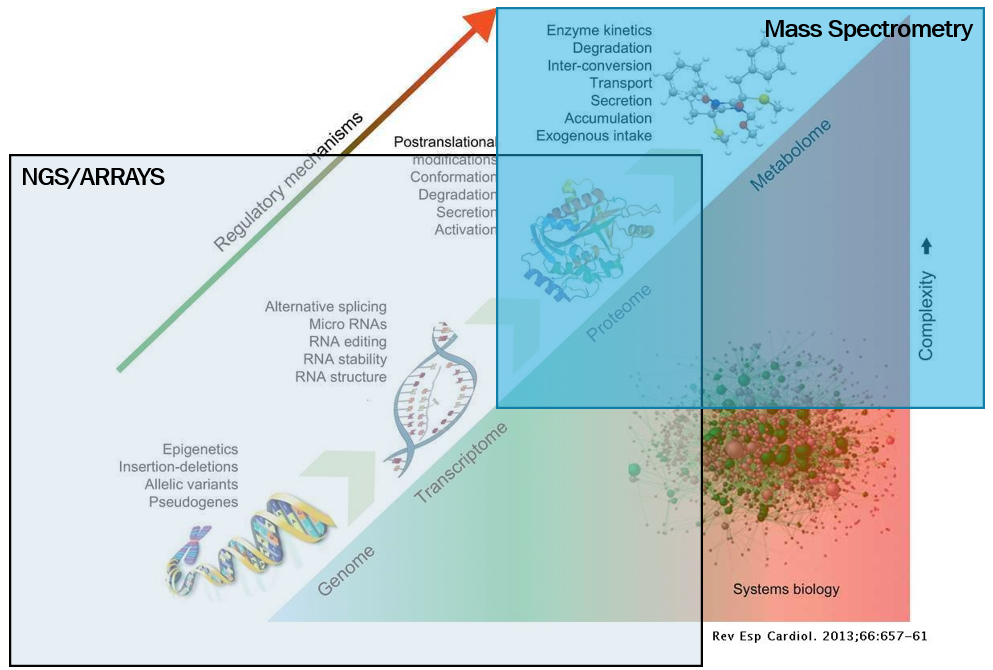
\includegraphics[width = 0.6\textwidth]{figs/omics.png}
\end{figure}

La genómica, transcriptómica y proteómica se pueden analizar utilizando tecnologías de secuenciación de próxima generación (NGS) y microarrays. Sin embargo, la proteómica y la metabolómica también se estudian comúnmente con espectrometría de masas, una técnica que permite identificar y cuantificar moléculas basándose en su masa y carga. Aunque la espectrometría de masas ofrece un mayor detalle en la identificación de proteínas y metabolitos, la secuenciación es más escalable y se está popularizando, especialmente en estudios a gran escala. Dos empresas comerciales que permiten la secuenciación de proteínas son Olink y Somalogic.

\section{Pipeline de un experimento ómico}
El pipeline de un experimento ómico aplica tanto a la cuantificación de la expresión génica con NGS, como a la identificación de proteínas con espectrometría de masas o de metabolitos con espectrometría. El proceso generalmente sigue los siguientes pasos:
\begin{enumerate}
\item \textbf{Pregunta biológica}: Todo experimento ómico comienza con una pregunta biológica clara. Esta pregunta debe ser lo suficientemente específica para guiar el diseño experimental y la elección de la plataforma tecnológica. Por ejemplo, si la pregunta es sobre la expresión génica en una cohorte grande de pacientes, la secuenciación de ARN (RNA-seq) podría ser la opción más adecuada.
\item \textbf{Elección de la plataforma tecnológica}: La elección de la tecnología (NGS, espectrometría de masas, microarrays, etc.) debe basarse en la pregunta biológica y no al revés. Por ejemplo, si se busca un alto rendimiento y escalabilidad, la secuenciación podría ser preferible sobre la espectrometría de masas.
\item \textbf{Diseño experimental}: Es crucial diseñar el experimento de manera que se minimice el sesgo y se maximice la reproducibilidad. Esto incluye la selección adecuada de controles, la replicación biológica y técnica, y la consideración de factores de confusión.
\item \textbf{Adquisición de datos}: Una vez diseñado el experimento, se procede a la recolección de datos. Esto puede implicar la secuenciación de ARN, la identificación de proteínas por espectrometría de masas, o la cuantificación de metabolitos.
\item \textbf{Preprocesamiento de datos}: Los datos crudos suelen requerir un preprocesamiento que incluye la corrección de errores, la normalización y la eliminación de ruido. Este paso es crucial para asegurar que los datos sean de alta calidad antes de proceder al análisis.
\item \textbf{Análisis de datos}: El análisis de datos en estudios ómicos generalmente incluye:
\begin{itemize}
\item \textbf{Identificación de genes diferencialmente expresados}: Esto implica comparar los niveles de expresión génica entre diferentes condiciones (por ejemplo, tejido sano vs. tejido enfermo) para identificar genes que están regulados al alza o a la baja.
\item \textbf{Análisis de clusters}: Este método agrupa genes o muestras con patrones de expresión similares, lo que puede ayudar a identificar subtipos de enfermedades o vías biológicas relevantes.
\item \textbf{Ingeniería reversa de redes génicas}: Este enfoque intenta reconstruir las redes de regulación génica a partir de los datos de expresión, lo que puede proporcionar insights sobre cómo los genes interactúan entre sí.
\end{itemize}
\item \textbf{Estandarización y almacenamiento de datos}: Los datos deben ser estandarizados y almacenados en bases de datos públicas o privadas para su posterior acceso y análisis. Una base de datos importante es el \textit{Gene Expression Omnibus (GEO)}, que alberga datos de expresión génica de diversos organismos y condiciones experimentales.
\item \textbf{Integración e interpretación biológica}: Finalmente, los datos se integran con información biológica adicional (como anotaciones funcionales, interacciones proteína-proteína, etc.) para interpretar los resultados en un contexto biológico más amplio. Esto puede llevar a la identificación de biomarcadores, dianas terapéuticas o mecanismos moleculares subyacentes a una enfermedad.
\end{enumerate}

\section{Diseño experimental}
El diseño experimental es esencial en estudios ómicos debido al alto coste de los experimentos. El objetivo es minimizar el coste y maximizar la información obtenida. Para lograrlo, hay dos aspectos clave:
\begin{enumerate}
\item \textbf{Pregunta biológica:} Es imprescindible tener una pregunta biológica clara y específica. Esto determina si el enfoque es \textit{data-driven} (exploratorio) o \textit{hypothesis-driven} (basado en hipótesis).
\item \textbf{Conocimiento de la tecnología:} Es crucial entender las limitaciones y capacidades de la tecnología utilizada. Esto incluye la precisión de las mediciones, la replicación y la identificación de variables que pueden introducir sesgos o variabilidad técnica. 
\end{enumerate}

En un experimento, hay dos tipos de errores:
\begin{itemize}
\item \textbf{Errores aleatorios:} No son predecibles, pero se pueden minimizar mediante la repetición de las mediciones.
\item \textbf{Errores sistemáticos:} Son predecibles y se pueden eliminar mediante la normalización o calibración de los datos.
\end{itemize}

Los principios para minimizar errores son:
\begin{enumerate}
\item \textbf{Replicación:} Incluye réplicas técnicas (para minimizar errores aleatorios) y réplicas biológicas (para asegurar que los resultados sean extrapolables a la población). La distinción entre réplicas biológicas y técnicas depende de qué fuentes de variación se estudien o, alternativamente, se consideren fuentes de ruido. Existen las réplicas técnicas, las cuales minimizan los errores aleatorios mediante el promedio y ayudan a testar la tecnología, y réplicas biológicas, que permiten sacar conclusiones extrapolables a la población completa y no solo del individuo, además de poder controlar la variabilidad en diferentes pasos experimentales.
\item \textbf{Randomización:} Asegura que las muestras sean representativas de la población.
\item \textbf{Blocking:} Reduce fuentes conocidas de variación que no son relevantes para la pregunta biológica.
\end{enumerate}

\subsection{Ejemplo de diseño experimental}
Supongamos que se mide la expresión de un gen en células de hígado de ratón, pudiendo realizar solo 48 mediciones. Se pueden considerar tres fuentes de variabilidad:
\begin{itemize}
\item \textbf{Replicación biológica}: se utilizan varios ratones, habiendo variabilidad entre los diferentes animales.
\item \textbf{Replicación entre biológica y técnica}: se escogen varias células de cada raón.
\item \textbf{Replicación técnica}: se realizan varias mediciones de cada célula. Las distintas mediciones de una misma célula deberían ser similares.
\end{itemize}
Si se realiza la media de los tres ratones, la medida va a ser muy variable en relación con una sola medida, pero esto sirve para el test estadístico, ya que son medidas independientes. En caso de tener medidas dependientes, no se puede utilizar la variabilidad para estudiar la significancia, ya que son medidas repetidas. 

Como en este modelo propuesto hay que cuantificar la variabilidad, se pueden realizar simulaciones para determinar el número óptimo de réplicas biológicas y técnicas para minimizar la variabilidad y maximizar la precisión.

\begin{figure}[h]
\centering
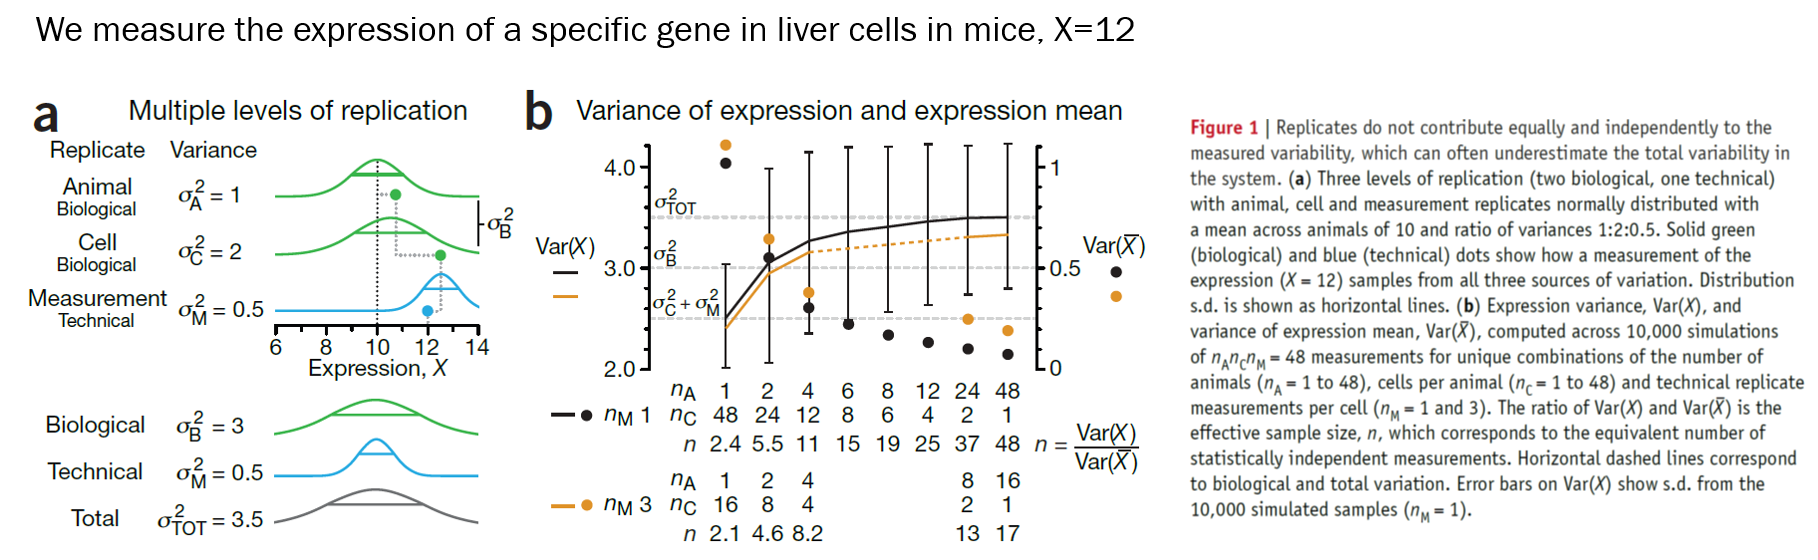
\includegraphics[width = \textwidth]{figs/replicates.png}
\end{figure}

En este experimento de ómicas, la expresión de un gen de células de hígado de ratón se cuantifica en 12. Las tres fuentes de variabilidad (animal, célula y medición) suman un 3,5. Las normales están centradas en 10, ya que las medidas están saliendo en ese valor, no en 12. Hay más variabilidad biológica que técnica, transformando las gaussianas en una campana más aplastada. Se realizaron simulaciones cambiando el número de animales, el número de células y el número de réplicas técnicas. Se hacen 10.000 asignaciones, para que se agrupen de forma diferente las combinaciones del número total (48 animales, 1 sola célula; 24 animales, 2 células; ...; 1 animal, 48 células). Sabiendo la cantidad de animales, células y mediciones, se puede sacar el tamaño muestral real del experimento, permitiendo calcular así la diferencia entre la variabilidad experimental y la variabilidad real. En ómicas, somos poco capaces de estimar la variabilidad, ya que en general hay pocas réplicas. Si esto después de mete en un t-test, y la variabilidad es muy pequeña (o incluso 0), entonces el resultado es muy grande, teniendo un p muy pequeño, rechanzando la hipótesis nula de que no hay diferencia en la expresión.

Para tecnologías ómicas, se deben incluir al menos 3 réplicas biológicas. Todo esto es para la experimentación con animales. En caso de experimentación en humanos, la variabilidad es gigante. 

\subsection{Réplicas vs profundidad}
Cuando comenzó la secuenciación, cuanto más se secuencie, más caro es el experimento. Por tanto, ¿es mejor más réplicas a menos profundidad, o menos réplicas a más profundidad? Hubo varios estudios con muchas simulaciones que vieron que lo importante era la secuenciación con réplica biológica. El número de lecturas tiene algo de relevancia, pero llegados a un número, no compensa a hacer mucha más secuenciación porque se llega a un plateau en cuanto a genes diferencialmente expresados. Las métricas aumentan más teniendo varias réplicas biológicas que teniendo varias lecturas. 

\begin{figure}[h]
\centering
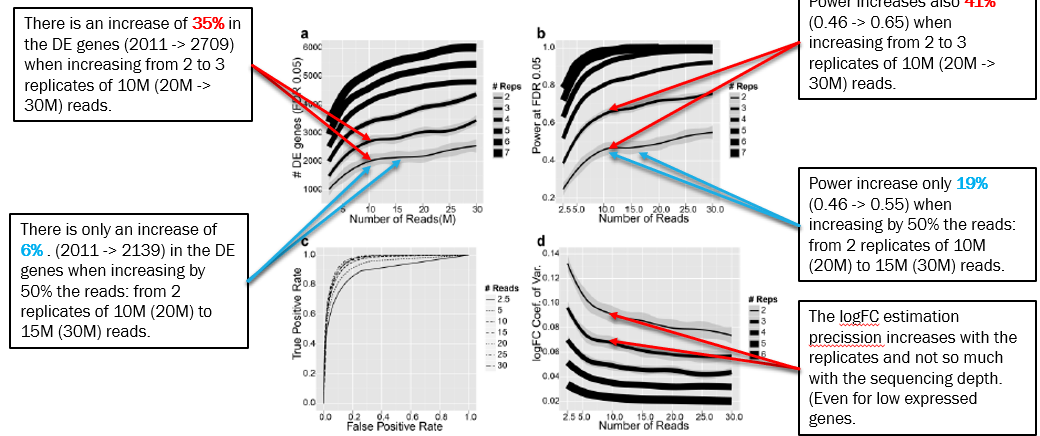
\includegraphics[width = \textwidth]{figs/replicates-depth.png}
\end{figure}

\subsection{Pooling, batch y blocking}
En el contexto de los experimentos ómicos, el \textbf{pooling} es una estrategia que consiste en combinar (o "agrupar") múltiples muestras biológicas en una sola muestra antes de realizar el análisis. Esta técnica se utiliza principalmente para reducir costes y simplificar el procesamiento de muestras, especialmente cuando se trabaja con un gran número de individuos o cuando los recursos económicos son limitados. En lugar de analizar cada muestra individualmente, se mezclan varias muestras en una sola. Por ejemplo, si tienes 12 muestras de ARN de diferentes individuos, podrías combinarlas en 3 grupos (pools) de 4 muestras cada uno. Una vez combinadas, las muestras agrupadas se procesan y analizan como una sola. Esto significa que, en lugar de obtener datos individuales para cada muestra, obtienes un resultado promedio para cada pool. En el caso de muestras humanas no se hace porque se pierde información individual fenotípica y genotípica, pero en animales sí puede ser una buena idea si las características específicas por especimen (sexo, camada, edad, etc.) no son relevantes para el experimento. Lo mejor es tener cuantas más réplicas independientes posibles. 

\begin{figure}[h]
\centering
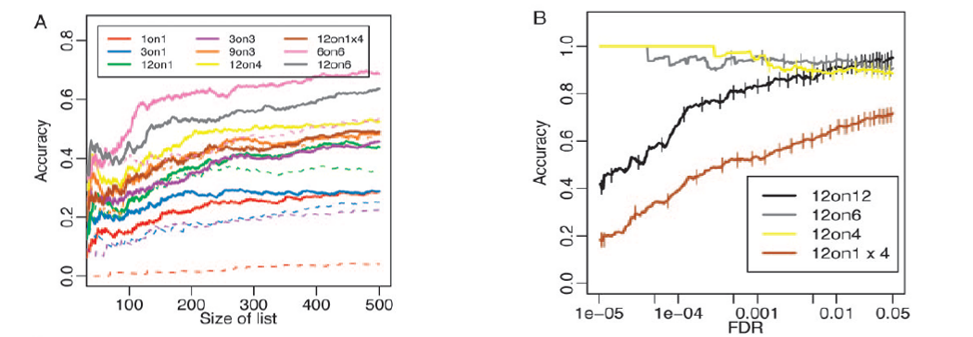
\includegraphics[width = 0.9\textwidth]{figs/pooling.png}
\end{figure}

Algunos pasos en los que se introduce variabilidad en NGS son:
\begin{itemize}
\item Técnica: extracción del ARN, preparación de la librería, flow-cell, barcode, científico
\item Biológica: sexo, camada/familia, edad
\end{itemize}
Además, hay sesgos sistemáticos y ruido por errores aleatorios.

Cuando los experimentos se realizan en varias tandas (por ejemplo, por ser estudios muy grandes con muchas muestras), es crucial controlar el \textbf{efecto de batch} \marginpar[\footnotesize !!!!!]  \ para evitar sesgos técnicos. Esto se puede lograr mediante la randomización de muestras entre batches y el uso de modelos estadísticos mixtos.
Nunca hay que confundir el batch con el grupo biológico relevante, ya que es imposible ver si las diferencias son debidas al grupo biológico o a la variabilidad técnica. Cuando hay condiciones biológicas muy fuertes, a veces no se ven, pero si se hacen todas las muestras de una condición en un mismo batch, probablemente se estén magnificando las diferencias observadas. Por tanto, no hay que medir las distintas condiciones biológicas en batches distintos, si no mezclar en un batch muestras de distintas condiciones biológicas para poder utilizar la variable batch en el modelo estadístico mixto, normalizando por las diferencias entre los batches.

\begin{figure}[h]
\centering
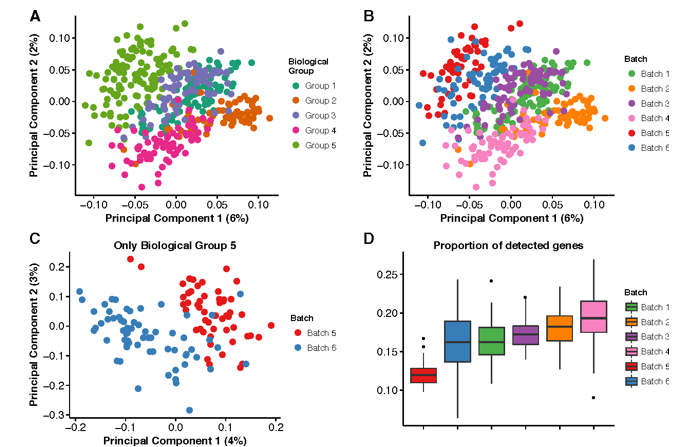
\includegraphics[width = 0.7\textwidth]{figs/batch.png}
\end{figure}

El \textbf{blocking} reduce fuentes conocidas e irrelevantes de variación entre unidades, permitiendo una precisión mayor en la estimación de las fuentes de variación estudiadas. Minimiza el efecto de variables de tipo biológico o técnico, que no son relevantes para la pregunta biológica. Una forma de hacer blocking secuenciando es metiendo adaptadores para hacer un barcoding de cada muestra, preparar la librería con todo junto y crear, de esa muestra, las distintas alícuotas a secuenciar. De esta forma se reduce el efecto de línea.

\begin{figure}[h]
\centering
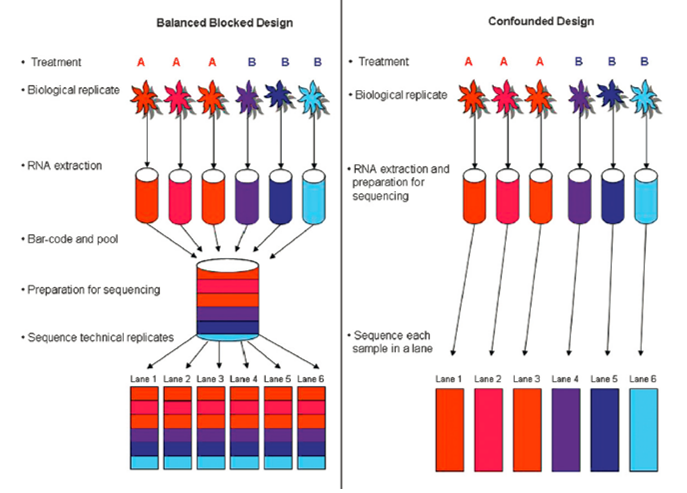
\includegraphics[width = 0.5\textwidth]{figs/blocking.png}
\end{figure}

\subsection{Diseño experimental - Ejercicios}
\subsubsection{Ejercicio de animales}
Tenemos un ratón knock-out en la proteína Bmi1. Para cada camada tenemos varios ratones WT y KO. Queremos encontrar metabolitos cuya expresión cambie significativamente entre condiciones
Disponemos de 6 camadas con el siguiente número de animales:
\begin{table}[h]
\centering
\begin{tabular}{c | c c}
Camada & KO & WT \\ \hline
L1 & 1 & 2 \\
L2 & 2 & 2 \\
L3 & 1 & 1 \\
L4 & 1 & 3 \\
L5 & 2 & 3 \\
L6 & 3 & 2 
\end{tabular}
\end{table}

\begin{itemize}
\item \textbf{Caso 1: No hay limitación económica}: se secuencia todo, ya que cuantas más muestras independientes, mejor.
\item \textbf{Caso 2: Se pueden secuenciar un máximo de 6 muestras}: De las 6 camadas se escogen aleatoriamente 3, de las cuales escoger un ratón KO y uno WT. Otra opción es coger las camadas 2 y 3 y secuenciar todos esos individuos. En este caso, como las camadas tienen efecto, se podría elegir un individuo de cada camada y hacer pool de 2 en 2. 
\item \textbf{Caso 3: L5 no tiene ningún animal KO y seguimos con el máximo de 6 muestras}: L5 no se tendría en cuenta porque podría introducir sesgos (quizás el KO no ha salido, o quizás no es viable), y del resto de camadas se escogen 3 camadas al azar para seleccionar un ratón de cada condición. Esto se debe a que no se podría comparar el pool entre la misma camada con pool entre distintas camadas.
\item \textbf{Caso 4: máximo de 6 muestras si no hay efecto de la camada}: se mezclan todos los ratones de las distintas camadas, separando por condición biológica, y se sacan 3 de cada uno al azar. Se podrían coger 12 y 12 y pooles de 4, o 6 y 6 y pooles de 2.
\end{itemize}

\subsubsection{Ejercicio de humanos}
Tenemos una cohorte de 100 muestras humanas con diabetes. Queremos probar en ellas un fármaco y ver sus efectos en la expresión génica. Podemos secuenciar un total de 40 muestras. Por estudios piloto sabemos que el sexo y el IMC afectan al impacto del fármaco. La composición de la cohorte es la siguiente:
\begin{table}[h]
\centering
\begin{tabular}{c | c c}
 & Hombres & Mujeres \\ \hline
IMC alto & 40 & 20 \\
IMC bajo & 20 & 20
\end{tabular}
\end{table}
Además, no podemos procesar todas las muestras juntas, tenemos que hacerlo en dos ejecuciones.
\begin{itemize}
\item \textbf{Q1: ¿Cómo se asignan los pacientes a los grupos fármaco y placebo?} Se escogen 5 personas de cada condición (sexo y BMI) para fármaco y otros 5 para placebo. 
\item \textbf{Q2: ¿Qué pacientes se secuenciarían en cada turno?} Se cogen ordenadamente una muestra de cada grupo y condición.
\end{itemize}

%31/01 - Fátima
\section{Consideraciones estadísticas para datos ómicos}
\subsection{Ejemplo - Statistics for Omics}
En este ejemplo, se utilizan datos del paquete de R maPooling, que contiene información sobre la expresión génica en dos condiciones (por ejemplo, wild-type vs. knock-out) y diferentes animales de cada condición. La matriz de diseño indica qué ratones (columna) están incluidos en cada muestra (fila), con un 1 para los ratones incluidos y un 0 para los excluidos. Por ejemplo, a3tr1 representa una réplica técnica del ratón 3 de la condición a, y aq es un pool de todos los ratones de la condición a.

El siguiente código muestra qué ratones están incluidos en cada muestra:
\begin{lstlisting}[language=R]
# r
library(rafalib)
mypar()
flipt <- function(m) t(m[nrow(m):1,])
myimage <- function(m,...) {
  image(flipt(m),xaxt="n",yaxt="n",...)
}
myimage(as.matrix(pData(maPooling)),col=c("white","black"),
        xlab="experiments",
        ylab="individuals",
        main="phenoData")
\end{lstlisting}

\begin{figure}[h]
\centering
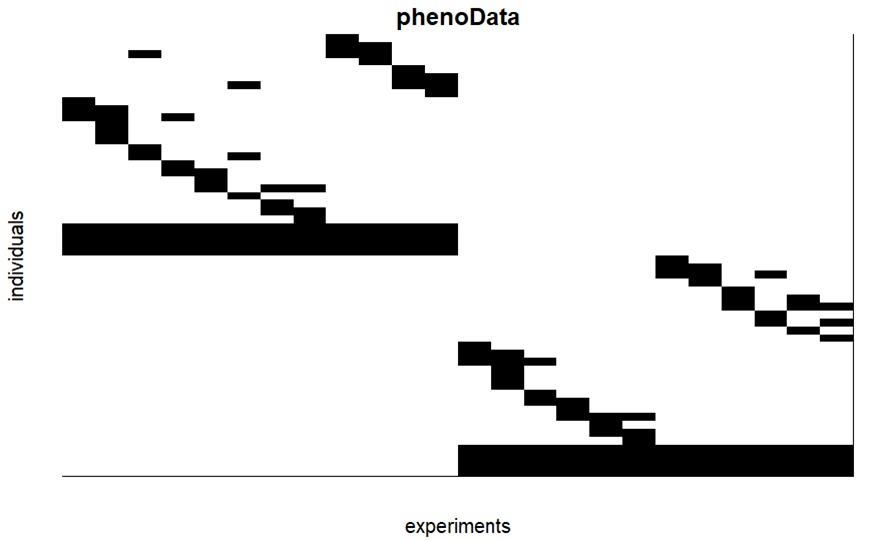
\includegraphics[width = 0.9\textwidth]{figs/pools.jpg}
\end{figure}

El objetivo es identificar diferencias en la expresión génica entre las condiciones a y b. Para ilustrar esto, se examinan dos genes específicos:
\begin{lstlisting}[language=R]
# r
###look at 2 pre-selected genes for illustration
i=11425;j=11878
pooled_y=exprs(maPooling[,pooled])
pooled_g=factor(as.numeric(grepl("b",names(pooled))))
mypar(1,2)
stripchart(split(pooled_y[i,],pooled_g),vertical=TRUE,method="jitter",col=c(1,2),
           main="Gene 1",xlab="Group",pch=15)
stripchart(split(pooled_y[j,],pooled_g),vertical=TRUE,method="jitter",col=c(1,2),
           main="Gene 2",xlab="Group",pch=15)
\end{lstlisting}

\begin{figure}[h]
\centering
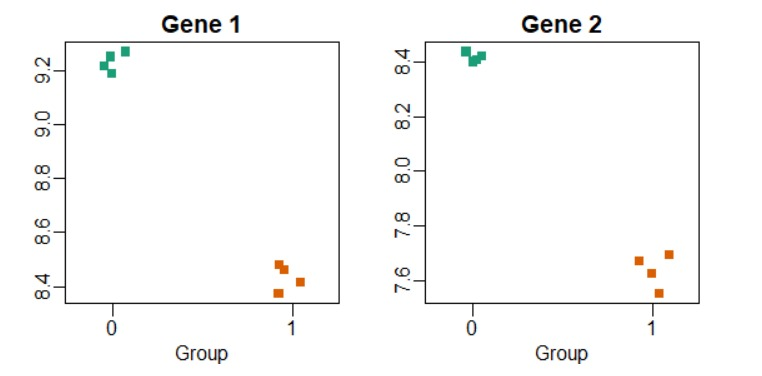
\includegraphics[width = 0.9\textwidth]{figs/expresion-genica.jpg}
\end{figure}

Se realiza un test estadístico (t-test) para evaluar si las diferencias en la expresión génica son significativas. Los p-valores obtenidos son muy bajos, del orden de $10^{-7}$:
\begin{lstlisting}[language=R]
# r
library(genefilter)
pooled_tt=rowttests(pooled_y,pooled_g)
pooled_tt$p.value[i]
pooled_tt$p.value[j]
\end{lstlisting}

Para obtener la variabilidad biológica, se eliminan las réplicas técnicas y se calcula la desviación estándar de las réplicas biológicas:
\begin{lstlisting}[language=R]
# r
technicalsd <- rowSds(pooled_y[,pooled_g==0])
biologicalsd <- rowSds(y[,g==0])
LIM=range(c(technicalsd,biologicalsd))
mypar(1,1)
boxplot(technicalsd,biologicalsd,names=c("technical","biological"),ylab="standard deviation")
\end{lstlisting}

\begin{figure}[h]
\centering
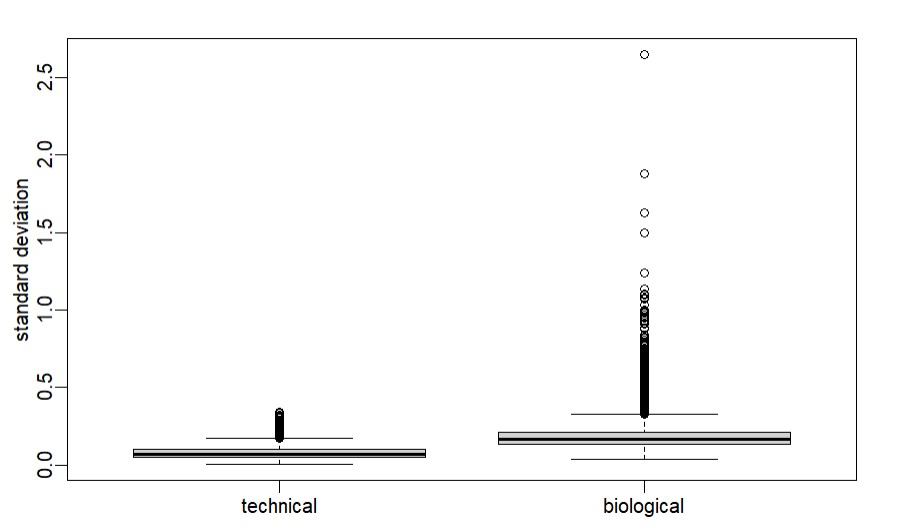
\includegraphics[width = 0.9\textwidth]{figs/variabilidad-biologica.jpg}
\end{figure}

Se observa que la variabilidad biológica es mucho mayor que la variabilidad técnica. Además, la variabilidad de las varianzas también es mayor para la variabilidad biológica. A continuación, se muestran los valores de expresión de los dos genes en cada ratón individual:
\begin{lstlisting}[language=R]
# r
mypar(1,2)
stripchart(split(y[i,],g),vertical=TRUE,method="jitter",col=c(1,2),xlab="Gene 1",pch=15)
points(c(1,2),tapply(y[i,],g,mean),pch=4,cex=1.5)
stripchart(split(y[j,],g),vertical=TRUE,method="jitter",col=c(1,2),xlab="Gene 2",pch=15)
points(c(1,2),tapply(y[j,],g,mean),pch=4,cex=1.5)
\end{lstlisting}

\begin{figure}[h]
\centering
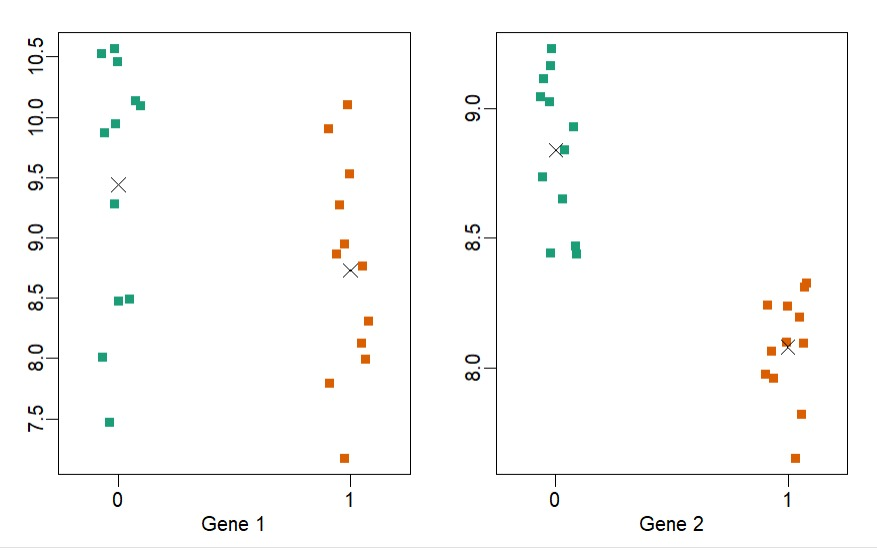
\includegraphics[width = 0.9\textwidth]{figs/expresion-genica2.jpg}
\end{figure}

Al volver a calcular el t-test, se observa que el gen 1 no es significativo, mientras que el gen 2 sí lo es:\begin{lstlisting}[language=R]
# r
library(genefilter)
tt=rowttests(y,g)
tt$p.value[i]
tt$p.value[j]
\end{lstlisting}

\subsection{Estadística en datos ómicos}
En experimentos con animales, el número mínimo recomendado de réplicas biológicas independientes es 3, que pueden incluir pooling (combinación de muestras). Sin embargo, en humanos, la variabilidad es mucho mayor, y el pooling no es recomendable debido a la pérdida de información individual.

Los experimentos ómicos se caracterizan por tener una \textbf{matriz "skinny}", es decir, muchas filas (genes, proteínas, metabolitos) y pocas columnas (muestras). Esto se conoce como la \textbf{maldición de la dimensionalidad} ("curse of dimensionality"). Aunque no es "Big Data" en el sentido estricto (ya que no hay muchas muestras), tener tantas características (filas) presenta desafíos estadísticos.

\subsubsection{Problemas con la estimación de la variabilidad}
Con pocas réplicas, la estimación de la variabilidad es imprecisa. En un t-test, se compara la diferencia de medias entre dos grupos en relación con la variabilidad dentro de cada grupo. Si la variabilidad se subestima, el t-test puede dar resultados falsamente significativos.

Para abordar este problema, se utiliza información de todo el experimento para estimar mejor la variabilidad. Esto se conoce como \textbf{moderación de la variabilidad o shrinkage}. La idea es "regularizar" la variabilidad utilizando la distribución de las desviaciones estándar de todos los genes. Por ejemplo:
\begin{itemize}
\item \textbf{Cálculo de la mediana:}  Se calcula la mediana de todas las desviaciones estándar y se añade un offset ($s_0$ ) a la estimación de la variabilidad de cada gen. Esto evita que valores extremadamente bajos de variabilidad (debidos al azar) dominen los resultados. 
\item \textbf{Uso del percentil 90:} En lugar de la mediana, se puede usar el percentil 90 de las desviaciones estándar para obtener estimaciones más conservadoras. Esto es útil porque los genes con variabilidades muy altas probablemente no sean reales. Y en ómicas, lo más importante es que lo que se estudie sea real. 
\end{itemize}
Este enfoque se implementa en métodos como el \textbf{t-test moderado} (por ejemplo, en el paquete limma de R), que ajusta las estimaciones de variabilidad para hacerlas más robustas.

El shrinkage es una técnica estadística que "contrae" las estimaciones de variabilidad hacia un valor central (como la mediana o el percentil 90). Esto ayuda a evitar sobreajustes y a obtener resultados más confiables en experimentos con pocas réplicas.

\subsubsection{Problema de la no normalidad de los datos ómicos}
Los datos ómicos (como los de expresión génica) a menudo no siguen una distribución normal, lo que puede complicar su análisis estadístico. Para abordar este problema, se utilizan técnicas de \textbf{transformación} y \textbf{normalización} de los datos, que permiten que estos se ajusten mejor a los supuestos de los tests estadísticos. Estas transformaciones pueden ser de dos tipos:
\begin{itemize}
\item \textbf{Normalizaciones interpretables:} Aquellas que buscan que los datos tengan un significado biológico claro.
\item \textbf{Normalizaciones estadísticas:} Aquellas que buscan estabilizar la varianza o cumplir con los supuestos de los tests estadísticos.
\end{itemize}

\paragraph{Estabilización de la varianza} Uno de los principales problemas en los datos ómicos es que la \textbf{variabilidad} no es constante en todos los niveles de expresión. En general, los genes poco expresados tienden a tener una variabilidad mucho mayor que los genes muy expresados. Esto puede sesgar los resultados de los tests estadísticos, ya que estos asumen que la varianza es homogénea.

Para solucionar este problema, se utiliza la estabilización de la varianza. Una herramienta común para esto es voom, que es parte del paquete limma en R. Voom transforma los datos de conteo de secuenciación (como los de RNA-seq) para estabilizar la varianza y hacer que los datos sean más adecuados para análisis estadísticos basados en modelos lineales.

\paragraph{Normalización por longitud del gen y tamaño de la librería} En los datos de secuenciación (por ejemplo, RNA-seq), hay dos factores importantes que deben tenerse en cuenta al comparar la expresión génica:
\begin{itemize}
\item \textbf{Longitud del gen:} Los genes más largos tienden a tener más lecturas (reads) simplemente porque hay más regiones donde las lecturas pueden alinearse. Para comparar la expresión entre genes de diferentes longitudes, es necesario normalizar por la longitud del gen. Esto se hace típicamente mediante métricas como FPKM (Fragments Per Kilobase of transcript per Million mapped reads) o TPM (Transcripts Per Million).
\item \textbf{Tamaño de la librería:} El número total de lecturas en una muestra (tamaño de la librería) puede variar entre condiciones experimentales. Si no se normaliza por el tamaño de la librería, las diferencias en la expresión génica podrían deberse simplemente a que una muestra tuvo más lecturas en general, en lugar de a cambios biológicos reales. Métricas como CPM (Counts Per Million) ayudan a corregir esto.
\end{itemize}

Cuando se comparan las mismas condiciones entre sí, la longitud del gen no es un problema (ya que es constante), pero el tamaño de la librería sí puede afectar los resultados y debe ser normalizado.

\subsubsection{Problema de hipótesis múltiples}
En los experimentos ómicos, se realizan miles de tests estadísticos simultáneamente (uno por cada gen, proteína o metabolito). Esto da lugar al problema de las comparaciones múltiples, que aumenta la probabilidad de obtener falsos positivos (es decir, rechazar la hipótesis nula cuando en realidad es verdadera).

\paragraph{Hipótesis nula} La hipótesis nula en este contexto es que no hay diferencia en la expresión de un gen entre las condiciones comparadas. Sin embargo, debido al gran número de tests realizados, es probable que algunos genes aparezcan como diferencialmente expresados simplemente por azar.

Para controlar el número de falsos positivos, se utilizan métodos de corrección de múltiples comparaciones. Algunos de los más comunes son: 
\begin{itemize}
\item \textbf{Corrección de Bonferroni:} Ajusta el nivel de significancia ($\alpha$) dividiéndolo por el número total de tests realizados. Es muy conservadora y puede reducir demasiado la potencia estadística.
\item \textbf{Control de la tasa de descubrimiento falso (FDR):} Controla la proporción esperada de falsos positivos entre los resultados significativos. Es menos conservadora que Bonferroni y se utiliza ampliamente en análisis ómicos. Solo se permite un 5\% de errores entre los genes que se seleccionan como diferencialmente expresados.
\item \textbf{Valores q:} Son una versión ajustada de los p-valores que tienen en cuenta la corrección por múltiples comparaciones. Un valor q < 0.05 indica que se espera que menos del 5\% de los resultados significativos sean falsos positivos.
\end{itemize}

\subsubsection{Tamaño del efecto vs significancia}
En el análisis de datos ómicos, es crucial diferenciar entre la significancia estadística y la importancia biológica de los cambios observados. Mientras que la significancia estadística nos dice si un resultado es probablemente real (es decir, no debido al azar), el tamaño del efecto nos indica cuán grande o relevante es ese cambio biológicamente.

\paragraph{Tamaño del efecto: $log_2(FC)$} El tamaño del efecto se mide comúnmente como el logaritmo en base 2 del cambio en la expresión ($log_2(FC)$, donde $FC$ es el "fold change" o cambio en la expresión). Este valor indica cuánto ha aumentado o disminuido la expresión de un gen entre dos condiciones. Por ejemplo:
\begin{itemize}
\item Un $log_2(FC) = 1$ significa que la expresión del gen se ha duplicado.
\item Un $log_2(FC) = - 1$ significa que la expresión del gen se ha reducido a la mitad.
\end{itemize}

Los datos suelen transformarse a $log_2$ por dos razones principales:
\begin{itemize}
\item \textbf{Normalización:} La transformación logarítmica ayuda a estabilizar la varianza y hace que los datos se ajusten mejor a los supuestos de los tests estadísticos.
\item \textbf{Interpretabilidad:} Los valores en $log_2$ son más fáciles de interpretar, ya que los cambios se expresan en términos de duplicaciones o reducciones a la mitad.
\end{itemize}

\paragraph{Importancia del $log_2(FC)$} En cualquier experimento, es esencial examinar tanto el p-valor ajustado (que indica significancia estadística) como el $log_2(FC)$ (que indica el tamaño del efecto). Sin embargo, el umbral para considerar un $log_2(FC)$ como biológicamente relevante puede variar dependiendo del contexto experimental. Por ejemplo:
\begin{itemize}
\item En algunos casos, un $log_2(FC)$ pequeño (por ejemplo, 0.5) puede ser biológicamente relevante si afecta a genes clave en una vía importante.
\item En otros casos, solo cambios grandes (por ejemplo, $log_2(FC) > 1$) pueden considerarse relevantes.
\end{itemize}

Dependiendo del experimento, puede ser o no interesante filtrar los resultados por el $log_2(FC)$:
\begin{itemize}
\item \textbf{Interpretación individual de genes:} Si el objetivo es identificar genes individuales con cambios grandes en la expresión, es útil filtrar por $log_2(FC)$. Por ejemplo, se podría considerar solo aquellos genes con $|log_2(FC)| > 1$.
\item \textbf{Interpretación de grupos de genes:} Si el objetivo es analizar vías o grupos de genes (por ejemplo, mediante análisis de enriquecimiento funcional), puede no ser necesario filtrar por $log_2(FC)$. En este caso, incluso cambios pequeños en múltiples genes de una misma vía pueden ser biológicamente relevantes.
\end{itemize}

\subsection{Continuación ejemplo - Statistics for Omics}
Generamos nuestra propia distribución nula. Se asigna aleatoriamente 0 y 1 a cada una de las columnas.  Para esta nueva expresión barajada, se realiza el t-test para ver cuántos salen diferencialmente expresados.
\begin{lstlisting}[language=R]
# r
set.seed(0)
shuffledIndex <- factor(sample(c(0,1),sum(g==0),replace=TRUE ))
nulltt <- rowttests(y[,g==0],shuffledIndex)
NfalselySigAt01 = sum(nulltt$p.value<0.01)
NfalselySigAt01 #11
NfalselySigAt05 = sum(nulltt$p.value<0.05)
NfalselySigAt05 #201 falsamente significativos
\end{lstlisting}

En lugar del p-valor, vamos a calcular el q-valor, y comprobamos que efectivamente no sale ningún gen significativo.
\begin{lstlisting}[language=R]
# r
library(qvalue)
nullqvals = qvalue(nulltt$p.value)$qvalue
sum(nullqvals<0.05) #0
sum(nullqvals<0.01) #0
\end{lstlisting}

\subsection{Ejemplo inferencia}
Este ejemplo se basa en el paper "A Model for Studying Mechanisms and Treatment of Impaired Glucose Tolerance and Type 2 Diabetes". Script en carpeta de prácticas de la asignatura.
En el CSV mice\_pheno se muestra el sexo, dieta y peso de los ratones. El experimento está bastante equilibrado: 225 hembras con dieta control, 200 hembras con dieta grasa, 224 machos con dieta control y 197 machos con dieta grasa.

Hay varias representaciones. Entre ellas, el barplot es una figura muy poco explicativa. El boxplot es algo más indicativo, mostrando que hay poca diferencia entre los dos grupos de dietas al cruzarse las barras de error.

Como los ratones machos suelen ser más grandes (y por tanto, más pesados) que las ratonas hembra, solo seleccionamos a las últimas. Tras volver a hacer el boxplot, vemos que las medias no están tan desencaminadas, pero la variabilidad es mucho más grande que con toda la población. A continuación se muestrean 12 ratones con dieta control y 12 ratones con dieta alta en grasas de la población total. 

Se realiza lo mismo para 1000 muestras y se simula la distribución con 5 réplicas en lugar de 12, siendo el resultado una distribución más amplia (hay más variabilidad si se tienen menos réplicas). 

En ómicas, como hay muchos datos, se puede simular cómo sería la distribución nula y comparar si hay una diferencia real entre los grupos.